\section{\label{I-C-1}L'arbre de Porphyre: origines et influences}
\titreEntete{L'arbre de Porphyre: origines et influences}

%intro
La définition d'un terme est une réflexion millénaire, et la recherche d'un référentiel, d'un dictionnaire pur n'est toujours pas abouti --- l'intelligence artificielle nécessitant des référentiels solides, la réflexion sur la pureté du dictionnaire utilisé est constante. \nP{Umberto}{Eco} considère que le dictionnaire \og ne devrait comporter, pour la définition d'un  terme, que les propriétés nécessaires et suffisantes pour distinguer ce concept d'un autre\fg\footcite[chap.1]{eco_arbre_2010}. Ces propriétés nécessaires à la définition du terme ne doivent pas être une connaissance du monde, mais bien des propriétés analytiques: \og Animal\fg{} est une propriété analytique de \og Chien\fg{} alors que l'aboiement est une connaissance.\\

La théorisation du dictionnaire remonte à l'Antiquité et a eu de nombreuses influences dans les systèmes classificatoires jusqu'à nos jours: les vocabulaires utilisés en institutions patrimoniales sont pour la plupart des hiérarchies de termes.

\subsection{\label{I-C-1-a}L'arbre de Porphyre}
\titreEntete{L'arbre de Porphyre}

La pensée aristotélicienne considère la définition d'un terme comme la forme substantielle, c'est à dire les attributs essentiels: l'\og homme\fg{} est un \og Animal rationnel mortel\fg{}\footcite[chap.1]{eco_arbre_2010}. L'assemblage de ces propriétés essentielles créé une définition, mais chacune de ces propriétés peut s'appliquer à d'autres entités. \\

Le commentateur des \textit{Catégories} d'Aristote au \textsc{III}\textsuperscript{ème}siècle, Porphyre, établit des arbres pour décrire le monde: celui des \og Substances\fg{} a le plus de postérité en étant \og un ensemble hiérarchisé et fini de genres et de substances\fg{}\footcite[chap.1]{eco_arbre_2010}, partant du \textit{Summus genus}, la Substance, pour atteindre une espèce indivisible, définie uniquement par ses attributs analytiques appelés genres\footnote{Voir \reference{arbre_porphyre_analytique}}. Un arbre de Porphyre est par conséquent une succession de genres divisés en espèces qui deviennent elles-mêmes des genres.\\

\begin{figure}[!h]
	\centering
	\Tree[.\textsc{Substance} 
		Incorporelle
		[.Corporelle 
			{Non vivante}
			[.Vivante 
				{Non animale}
				[.Animale 
					[.\textbf{Homme/Cheval} ]]]]]
	
	\caption[Arbre porphyrien de l'homme avec les seuls attributs analytiques]{Arbre porphyrien de l'homme avec les seuls attributs analytiques [d'après \cite{eco_arbre_2010}]}
	\label{arbre_porphyre_analytique}
\end{figure}

L'impossibilité de la distinction entre l'homme et le cheval impose de tenir compte des différences qui ne sont pas des attributs analytiques: \og La rationalité est la différence de l'homme\fg{}\footcite[chap.1]{eco_arbre_2010}. Ainsi, ces différences vont s'ajouter aux genres des espèces. Ces différences deviennent elles-mêmes divisibles et constitutives: elles deviennent genre. Ces différences sont essentielles pour distinguer une espèce d'une autre (voir \reference{arbre_porphyre_differences}).\\

\begin{figure}[!h]
	\centering
	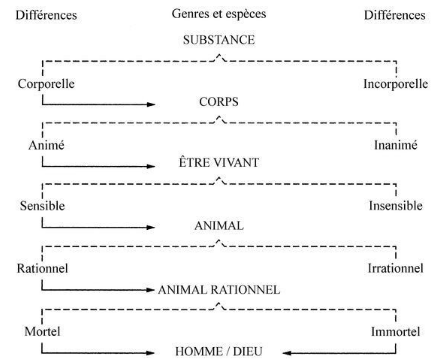
\includegraphics[width=12cm]{images/arbre_porprhyre_differences.png}
	\caption[Arbre porphyrien prenant en compte les différences]{Arbre porphyrien prenant en compte les différences [Source: \cite[chap.1]{eco_arbre_2010}]}
	\label{arbre_porphyre_differences}
\end{figure}

Cependant, si la prise en compte des différences permet de différencier l'homme du cheval, elles ne permettent pas de distinguer le cheval de l'âne par exemple. Un même genre doit donc être utilisé plusieurs fois dans l'arbre, ce qui le rend infini, et l'établissement d'un dictionnaire impossible à réaliser (voir \reference{arbre_porphyre_boucle}).\\

\begin{figure}[!h]
	\centering
	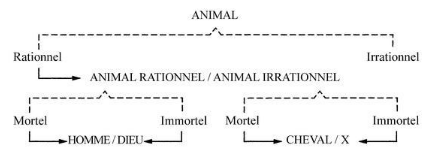
\includegraphics[width=12cm]{images/arbre_porphyre_boucle.png}
	\caption[Infinitude de l'arbre de Porphyre]{Infinitude de l'arbre de Porphyre [Source: \cite[chap.1]{eco_arbre_2010}]}
	\label{arbre_porphyre_boucle}
\end{figure}

Face à cette impossibilité de décrire le monde avec des divisions uniques dans un seul arbre, c'est à dire d'établir un dictionnaire universel, absolu et global, la seule solution paraît être la création d'un nombre d'arbres infini, composés de propriétés s'articulant selon le contexte et le domaine d'utilisation de l'arbre: d'un seul arbre insaisissable, une forêt réorganisable à l'envi et à l'infini est apparue, laissant le choix à l'utilisateur de l'arbre utilisé selon le sujet.

\subsection{\label{I-C-1-b}L'encyclopédisme (Antiquité - Moyen-Âge): la recherche d'un arbre global mimant le monde réel}
\titreEntete{L'encyclopédisme}

L'utopie de saisie totale du monde se retrouve dans l'encyclopédisme, dès l'\textit{Historia naturalis} de \nP{Pline}{l'Ancien}. Sur le même principe que l'arbre porphyrien, la hiérarchie de l'index de cette encyclopédie de 37 volumes part de l'original vers le dérivé, du naturel à l'artifice: \og Une encyclopédie, pour s’organiser, tente de suivre le modèle de l’arbre --- qui est toujours plus ou moins consciemment celui de la subdivision binaire d’un arbre porphyrien\fg{}\footnote{\cite[chap.1]{eco_arbre_2010}. Voir \reference{index_pline}}. Cependant, l'index d'une encyclopédie se distingue des termes d'un arbre porphyrien en ce qu'il est défini dans un autre développement --- un article d'encyclopédie ---, alors que les termes de l'arbre de Porphyre ne peuvent pas être définis par la suite.

\begin{figure}[!h]
	\centering
	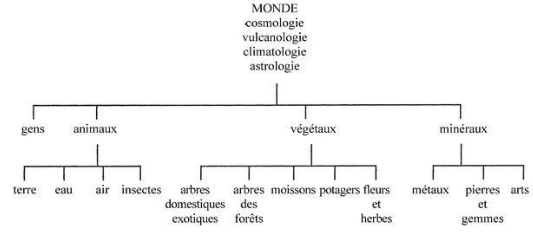
\includegraphics[width= 13cm]{images/index_pline.png}
	\caption{Extrait de l'arborescence de l'index de \nP{Pline}{l'Ancien}}
	\label{index_pline}
\end{figure}

Avec le passage au christianisme, l'encyclopédisme doit décrire les textes sacrés et non plus le monde. Ainsi, des éléments moralisateurs et allégoriques se retrouvent dans les index, devant les éléments matériels du monde\footnote{La tradition moralisatrice encyclopédique naît avec le \textit{Physiologos} d'un auteur grec et s'inspire de l'œuvre de \nP{Pline}{l'Ancien}, et se poursuit tout au long du Moyen-Âge avec les \textit{Étymologies} d'\nP{Isidore}{de Séville} notamment.}. À partir du \textsc{XIII}\textsuperscript{ème}siècle, les encyclopédies montrent l'ordre qui les dirige: cela conduit à \textit{L'arbre de science} de \nP{Raymond}{Lulle} qui créé seize arbres représentant l'Être, chacun représentant un savoir différent en se divisant en sept parties (racines, tronc, branches, rameaux, feuilles, fleurs, fruits)\footcite[chap.10]{eco_arbre_2010}. Contrairement à l'arbre de Porphyre qui est un arbre vide que l'on peut remplir selon le contexte, les arbres que propose \nP{Raymond}{Lulle} sont pleins et ont pour vocation de décrire et de classer le monde, la Grande Chaîne de l'Être.

\subsection{\label{I-C-1-c}Influences: une diversité de référentiels hiérarchiques}
\titreEntete{Influences: une diversité de référentiels hiérarchiques}

La pensée aristotélicienne puis le commentaire porphyrien ont produit une tradition de hiérarchisation du monde qui s'est poursuivie pendant plus d'un millénaire, sans cesse confrontée à l'impossibilité d'une description totale de ce monde. La multiplicité des arbres est, chez \nP{Umberto}{Eco} puis dans celle de \nP{Raymond}{Lulle}, la conclusion de leur réflexion. L'influence de cette tradition de description est sensible jusqu'à aujourd'hui, notamment dans le domaine de l'indexation et de la bibliothéconomie.\\

En effet, une diversité de référentiels est apparue, chacun étant dérivé d'un arbre. Des schémas de classification sont définissables à l'infini, emboîtant les genres, les espèces et les différences\footnote{\og Un simple artifice classificatoire consiste à emboîter des genres, des espèces et des différences sans en expliquer le \textit{definiendum}\fg{} in \cite[chap.1]{eco_arbre_2010}}. La taxonomie naît de ce modèle d'arbre: la taxonomie n'a pas pour but de dire comment repérer le concept décrit, elle permet seulement de classer en renvoyant, pour chaque nœud, vers un autre chapitre où l'on décrit ces propriétés. La taxonomie, bien qu'historiquement appliquée aux sciences de la terre, a été reprise par \nP{Melvil}{Dewey} dans sa classification décimale \index[referentiels]{dewey@Dewey} en 1876.\\

Définie comme un \og classement hiérarchique de termes préférentiels\fg{} par \nP{Louis}{Rosenfeld} et \nP{Peter}{Morville}\footcite{rosenfeld_information_2015}, la taxonomie ne veut pas définir, mais simplement permettre l'utilisation correcte et logique du terme par l'attribution de catégories et l'utilisation exclusive de relations hiérarchiques.\\

Les \textit{thesauri}\footnote{Ils sont décrits comme une \og liste organisée de termes contrôlées et normalisés (descripteurs et non-descripteurs) servant à l’indexation des documents et des questions dans un système documentaire\fg{} dans \cite{degez_thesauroglossaire_2001}. Peu formels, ils sont néanmoins le vocabulaire le plus utilisé pour l'indexation. L'un des \textit{thesauri} les plus utilisés est le \ac{gemet}(\cite{noauthor_general_nodate}). Le \index[referentiels]{gemet@GEMET} est disponible en plus de trente langues et diffusé par l'Agence européenne de l'Énergie. Voir \reference{I-C-2}.} utilisent plus de relations et de types de termes, de manière à indexer des contenus avec des mots-clés et à faciliter la recherche. Ce vocabulaire contrôlé hiérarchique reste proche du langage naturel en y intégrant les variantes, les synonymes, les descriptions, les traductions et les équivalences.\\

Pour avoir une plus grande formalisation du thésaurus, il faut utiliser une ontologie. Cette ontologie est la spécification formelle d'un espace de noms, d'un domaine particulier de la connaissance\footnote{L'une des ontologies les plus utilisées, notamment dans le web sémantique, est \ac{foaf}. \index[referentiels]{foaf@FOAF} permet la description précise des personnes. Voir \cite{noauthor_foaf_nodate}}. Elle identifie alors les objets à décrire, leurs relations au sein de ce domaine ainsi que leurs propriétés. L'ontologie n'est pas utilisée directement dans l'indexation ou la recherche, elle est d'abord utilisée pour instancier et raisonner, en s'éloignant du langage naturel avec l'utilisation d'identifiants techniques.\\

Les taxonomies, les \textit{thesauri} ainsi que les ontologies héritent tous du modèle de l'arbre, la description ou la classification par la hiérarchie étant la plus efficace pour ces besoins. Ces vocabulaires sont les plus complexes par les relations qui les composent. \nP{Louis}{Rosenfeld} et \nP{Peter}{Morville}\footnote{\cite{rosenfeld_information_2015}. Voir \reference{frise_voca}} considèrent l'anneau de synonymie comme le plus simple des vocabulaires, avec des relations d'équivalence, alors que les fichiers d'autorité et les taxonomies, fonctionnant sur la hiérarchie, sont plus complexes. Les \textit{thesauri} et les ontologies sont plus complexes encore puisqu'ils sont constitués de relations hiérarchiques et associatives.

\begin{figure}[!h]
	\centering
	
	\begin{pspicture}(0,2)(10,8)
		\psline[linewidth=1.5pt]{->}(0,5)(10,5)
		\uput[0](-2.5,5){\textsc{Simple}}
		\uput[0](10.5,5){\textsc{Complexe}}
		\uput[0](3,3){\textbf{\textsc{Type de relations}}}
		\uput[0](2.5,7){\textbf{\textsc{Type de vocabulaire}}}
		\uput[0](0,4){Équivalence}
		\uput[0](3.8,4){Hiérarchique}
		\uput[0](7.6,4){Associative}
		\uput[0](-1,6.3){Anneau de synonymie}
		\uput[0](2.5,5.5){Fichiers d'autorité}
		\uput[0](5,6.1){Taxonomies}
		\uput[0](7,5.5){Thésaurus}
		\uput[0](9,6.3){Ontologies}
	\end{pspicture}
	
	\caption[Classification des vocabulaires selon leur complexité]{Classification des vocabulaires selon leur complexité [d'après \cite{rosenfeld_information_2015}]}
	\label{frise_voca}
\end{figure}